\chapter{绘制端盖立体图}\label{chap:duangai}

{\bfseries 学习目标}
\begin{itemize}
\item 学习利用fillet命令绘制连接圆弧
\item 学习利用filletedge命令构建三维圆弧
\end{itemize}

{\bfseries 任务要求}
\begin{itemize}
\item 根据图\ref{fig:tiaoyafaduangai}所示的杯零件图,用旋转法建立调压阀杯零件的三维模型
\item 根据图\ref{fig:tiaoyafaduangai}所示的杯零件图,用实体建模法建立调压阀杯零件的三维模型
\end{itemize}

\noindent
\begin{figure}[htbp]
\centering
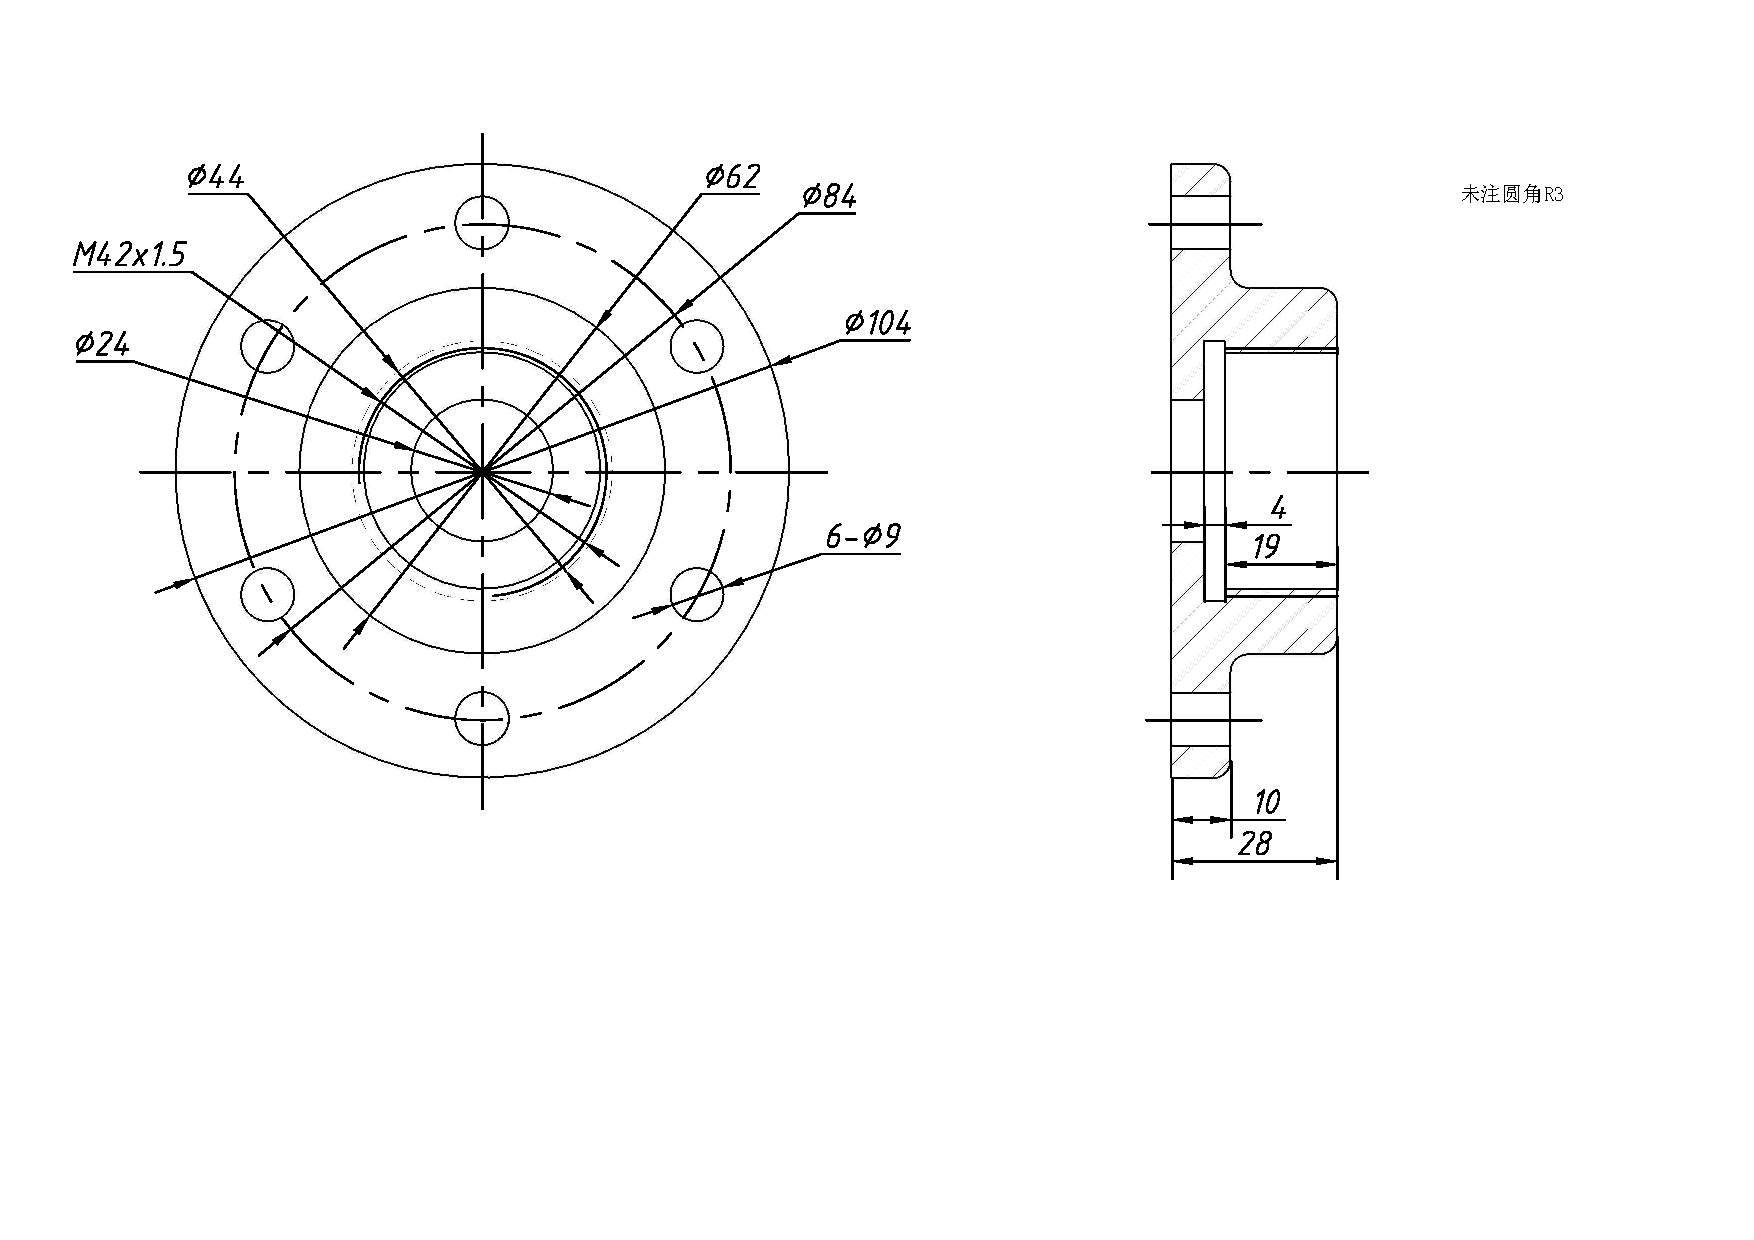
\includegraphics[scale=0.5]{tiaoyafaduangai.pdf}
\caption{端盖零件图}\label{fig:tiaoyafaduangai}
\end{figure}
\endinput